\documentclass[11pt,letterpaper]{article}
\usepackage[margin=1in]{geometry}
\usepackage{newtxtext,newtxmath}   % Times-compatible, as the course guide requires
\usepackage[T1]{fontenc}
\usepackage{microtype}
\usepackage{graphicx,booktabs,array,tabularx,xcolor,amsmath,enumitem}
\usepackage[most]{tcolorbox}
\usepackage[hidelinks]{hyperref}
\usepackage[font=small,labelfont=bf,labelsep=period,skip=6pt]{caption}
\usepackage[ruled]{algorithm}
\usepackage{algpseudocode}
\setlength{\parskip}{0.4em}\setlength{\parindent}{0pt}
\renewcommand{\arraystretch}{1.15}
\setlength{\textfloatsep}{12pt plus 2pt minus 2pt}
\setlength{\floatsep}{10pt plus 2pt minus 2pt}
\setlength{\intextsep}{10pt plus 2pt minus 2pt}
\renewcommand{\topfraction}{0.9}\renewcommand{\bottomfraction}{0.8}
\renewcommand{\textfraction}{0.1}\renewcommand{\floatpagefraction}{0.8}
\graphicspath{{figures/}}
\definecolor{abstractbg}{HTML}{EAF1FA}
\definecolor{abstractborder}{HTML}{B8C7DD}
\begin{document}
\thispagestyle{empty}
\begin{center}
{\LARGE\bfseries Detecting Logic Bugs in Relational Database Systems\par}
\vspace{4pt}
{\large Four oracles that compare a database with itself\par}
\vspace{12pt}
{\large\bfseries Group 12\par}
\vspace{4pt}
Fernando Berti Cruz Nogueira \quad Saatvik Paul \quad Haekwon Ahn\par
\vspace{2pt}
\small CSI 5137 A00 --- Advanced Topics in Databases and Data Management\\
Project 1 Report\par
\end{center}
\vspace{6pt}
\begin{tcolorbox}[enhanced,colback=abstractbg,colframe=abstractborder,boxrule=0.5pt,arc=4pt,
  left=10pt,right=10pt,top=10pt,bottom=10pt,title={\centering\bfseries Abstract},coltitle=black,
  colbacktitle=abstractbg,attach boxed title to top center={yshift=-2mm},boxed title style={colframe=abstractborder,boxrule=0pt,frame hidden,colback=abstractbg},
  fonttitle=\bfseries,boxsep=0pt]
\small
Logic bugs make a relational database return a wrong answer or keep a wrong state without crashing, so nothing signals the failure. This report reviews four papers from 2024--2025: CODDTest, DDLCheck, WriteCheck and Radar. Each detects such bugs by running two executions that should agree and flagging a mismatch, but they vary different things: expression evaluation, schema construction history, optional metadata, and transaction schedules. We compare their test oracles, equivalence assumptions, supported features and published experiments. The evaluations show that every method finds real bugs. Differences in workloads, DBMS versions, time budgets and confirmation procedures still rule out a ranking by bug count, so we compare the methods by the validity of their oracles and by what each one can and cannot reach.
\end{tcolorbox}
\vspace{8pt}
\begin{center}
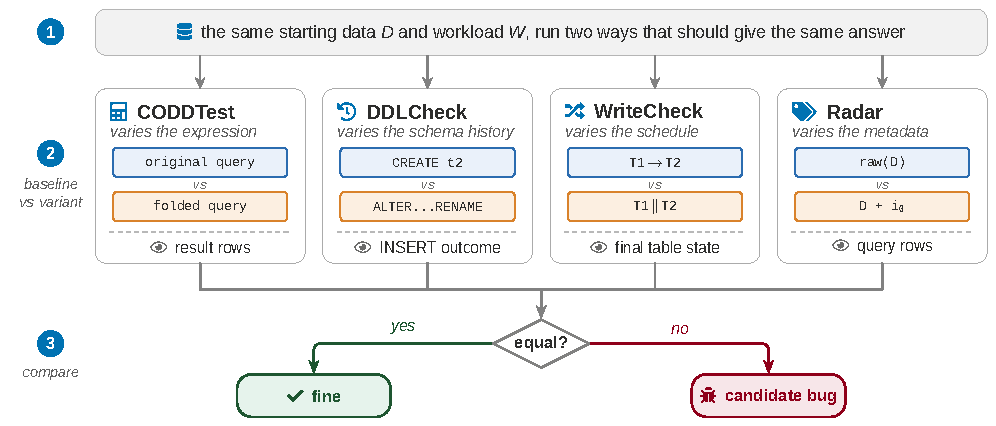
\includegraphics[width=\linewidth]{fig_overview}
\captionof{figure}{\textbf{Four oracles, one idea.} Each method runs two executions of the same data, here a table Product(id, quantity, reserved), that should give the same observable result: a folded expression versus the original query (CODDTest), a table built through ALTER statements versus built directly (DDLCheck), a concurrent schedule versus a serial one (WriteCheck), and a database with an index versus one without (Radar). A mismatch between the two observations is a candidate bug to be validated.}
\label{fig:overview}
\end{center}
\clearpage
% sec_a.tex: Introduction, Problem definition, Motivation, Related work

\section{Introduction}\label{sec:intro}
A database that crashes gets fixed the same day. A database that returns one wrong row can go unnoticed for years: the oldest bug CODDTest found had sat in MySQL for 14 years~\cite{coddtest}. These are \emph{logic bugs}. The system accepts a valid statement, reports success, and returns a wrong result or stores a wrong state, so the application has nothing to catch.

Finding them is hard because of the oracle problem. To see that an answer is wrong you need the right one, and writing a second SQL engine to compute it is out of reach. The four papers we review share a cheaper trick: ask the same system the same question in two ways that must agree. Figure~\ref{fig:oracles} shows one real bug per paper. CODDTest~\cite{coddtest} replaces an expression by its precomputed value. DDLCheck~\cite{ddlcheck} rebuilds a schema without its history. Radar~\cite{radar} drops optional metadata such as indexes. WriteCheck~\cite{writecheck} replays concurrent transactions one after another.

We ask how the equivalence each oracle relies on decides which bugs it can find, and how well each paper's experiments back its claims. The report contributes three things:
\begin{itemize}[leftmargin=1.1em,itemsep=1pt,topsep=2pt]
\item \textbf{One model for four oracles} (Section~\ref{sec:problem}, Figure~\ref{fig:model}).
\item \textbf{A coverage map} of the failures each oracle can observe (Table~\ref{tab:coverage}): each is strongest somewhere else, and all four share one blind spot.
\item \textbf{An evidence audit} (Sections~\ref{sec:experiments} and~\ref{sec:discussion}): verdicts per claim, and two reporting patterns that block any ranking by bug count.
\end{itemize}
All measurements come from the four papers; the model, matrices and verdicts are ours. NoREC and TLP~\cite{norec,tlp}, two earlier oracles, serve as background.

\section{Problem definition and discussion}\label{sec:problem}
\subsection{High-level description}
Picture a shop database with a \texttt{Product} table holding stock and reserved units. Whatever its past, some pairs of executions must agree. Replacing \texttt{quantity - reserved} by its value cannot change which products a query lists. A table created in its final form must behave like one that got there through three migrations. A query that never names an index must return the same rows with or without it. Two committed transactions must leave a state that some serial order could also produce. Logic-bug testing searches for inputs that break one of these promises.

\subsection{Formal definition and search objective}\label{sec:formal}
Let $E$ be a DBMS. A database state is $D=(S,V,M,H)$: visible schema $S$, stored values $V$, optional metadata $M$ such as indexes and constraints, and construction history $H$ with whatever hidden state it left. A workload $W$ is a query, a statement sequence or a set of transactions, and $C$ is the context (dialect, session settings, isolation level). The observation $O(E,D,W,C)$ is what the oracle compares: result rows, statement success, final contents or the schema. A transformation $T$ maps $(D,W)$ to $(D',W')$, and a precondition $P$ says when both pairs ask the same question.

\begin{tcolorbox}[enhanced,colback=panelbg,colframe=panelborder,boxrule=0.5pt,arc=3pt,left=7pt,right=7pt,top=4pt,bottom=4pt]
\small
\textbf{Given} $E$, $C$, a space of pairs $(D,W)$, a transformation $T(D,W)=(D',W')$ and a precondition $P$.
\textbf{Find} triples $(D,W,T)$ for which
\[
P(D,W,C)\;\wedge\;O(E,D,W,C)\not\equiv O(E,D',W',C),
\]
each reported with a reduced test case that reproduces it.
\end{tcolorbox}

Such a triple is a \emph{candidate}. It becomes a defect only after $P$ is confirmed, permitted nondeterminism is ruled out and the documentation is checked. The four papers do not use this notation; it is our common frame.

\subsection{Detailed discussion of the definition}\label{sec:detailed}
Each paper is one choice of $T$, $P$ and $O$, and Figure~\ref{fig:model} shows where each one intervenes. CODDTest and WriteCheck change the workload, DDLCheck the history, Radar the metadata. The precondition is what keeps each comparison honest. CODDTest needs a deterministic expression and a state that does not move between the auxiliary and the folded query. DDLCheck needs the rebuilt schema to match in every property later statements can see. Radar needs a read-only query that does not depend on what was dropped. WriteCheck needs writes that never use values read earlier in their transaction.

\begin{figure}[!tb]
\centering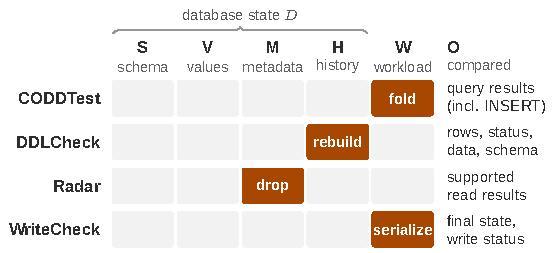
\includegraphics[width=\columnwidth]{fig_model}
\caption{\textbf{Where each oracle intervenes.} Orange marks the part of the state $D$ or the workload $W$ that the transformation changes; grey parts stay identical. The right column is the observation $O$ the oracle compares.}
\label{fig:model}
\end{figure}

\paragraph{What ``$\equiv$'' means.} Unordered results compare as multisets: order is ignored, duplicate counts are not, since a set would hide a dropped or duplicated row. NULLs, types, collation, rounding and errors need the same treatment on both sides, which is why CODDTest avoids extreme floating-point values and adds explicit casts in SQLite~\cite[Sec.~4.1]{coddtest}. For data-changing workloads, equal query output is not enough, because two INSERTs can both succeed and store different values. That is why DDLCheck and WriteCheck compare final state, and DDLCheck the schema too.

\subsection{Pseudoalgorithm}
Algorithm~\ref{alg:oracle} is the loop the four methods share. The real tools add steps: CODDTest runs an auxiliary query before folding, and WriteCheck must run the concurrent schedule before it knows which serial order to replay. Reduction (line~10) is the most underestimated step. Radar's authors spent three weeks reducing 1,663 raw reports to 42 unique bugs~\cite[Sec.~4.2]{radar}, and every shrink must keep the mismatch alive, because a smaller query can take a different plan and lose the bug.

\begin{algorithm}[!tb]
\caption{Generic metamorphic logic-bug search}
\label{alg:oracle}
\small
\begin{algorithmic}[1]
\Require DBMS $E$, context $C$, generator $G$, oracle family $F$, budget
\While{budget remains}
  \State $(D,W)\gets G.\textit{NextCase}(C)$
  \State $(T,P)\gets F.\textit{Choose}(D,W,C)$
  \If{\textbf{not} $P(D,W,C)$} \textbf{continue} \EndIf
  \State $(D',W')\gets T(D,W)$
  \State $A\gets\textit{RunFromCleanState}(E,D,W,C)$
  \State $B\gets\textit{RunFromCleanState}(E,D',W',C)$
  \If{\textbf{not} \textit{Equivalent}$(A,B,F.\mathit{rules})$}
    \State $\mathit{case}\gets\textit{ReduceKeepingMismatch}(D,W,T,C)$
    \State \textit{Record}$(\mathit{case},\text{version},\text{seed})$
  \EndIf
\EndWhile
\end{algorithmic}
\end{algorithm}

\begin{takeaway}
An oracle is a triple $(T,P,O)$. Each paper's contribution is a new transformation, the precondition that makes it safe, and an observation rich enough to show the bug.
\end{takeaway}

\section{Motivation}\label{sec:motivation}
\subsection{Running example}
Back to the shop. Each paper suggests a different test against \texttt{Product}. \textbf{Expressions:} filter on available stock, then rerun with the subquery replaced by its value. \textbf{History:} add \texttt{reserved} through \texttt{ALTER TABLE} and compare with a table created with it. \textbf{Metadata:} run the stock report with and without an index on \texttt{quantity}. \textbf{Transactions:} let two checkouts update \texttt{reserved} at once, then compare with a serial replay. One passing test says little about the others: an expression test on a fresh table never sees what a migration leaves behind, and a single-connection test never sees a write conflict. The transaction test needs care too. A checkout that reads \texttt{quantity} and later writes a value computed from it is outside WriteCheck's scope, and a race there is an application bug.

\subsection{Why it matters and what makes it hard}
DBMS developers receive short, reproducible cases that point at a wrong assumption in optimizer or executor code; CODDTest reports 33 of its 45 bugs fixed by publication~\cite{coddtest}. Application teams benefit because a wrong stored state outlives the request that caused it. Four things make the problem hard:
\begin{enumerate}[leftmargin=1.3em,itemsep=0pt,topsep=2pt]
\item \emph{Valid SQL is not a valid test.} A comparison needs a rule for NULLs, types, errors and nondeterminism.
\item \emph{The reference is not independent.} Both runs use the system under test, so a fault on both paths cancels out.
\item \emph{State is invisible.} Schema changes and metadata leave internal state that no query shows.
\item \emph{Concurrency has many right answers.} Choosing the serial order to compare against is itself a model.
\end{enumerate}

\subsection{Limitations of existing work, and can it be extended?}
Each paper narrows its comparison to make $P$ checkable, and each narrowing leaves a gap. \textbf{CODDTest} works on a fixed state; 4 of the 14 bugs it missed in its SQLite comparison involved indexes~\cite[Sec.~4.2]{coddtest}. \textbf{DDLCheck} needs a schema description complete enough to rebuild from; a lost property makes the reference wrong. \textbf{Radar} covers read-only queries, since dropping a UNIQUE constraint legitimately changes whether an INSERT succeeds. \textbf{WriteCheck} covers neither read-dependent writes nor read anomalies, and its serial order assumes a conflict model that semi-consistent reads and missing gap locks violate.

Can the gaps be closed? Partly. CODDTest's folding and Radar's raw copy both take a given state, so both could run on states that DDLCheck's histories produce, and DDLCheck already checks which of its bugs Radar could catch~\cite[Table~4]{ddlcheck}. WriteCheck is harder to extend: once a write uses a value read earlier, a serial replay may legitimately read something else, and the reference is no longer defined. None of these extensions is demonstrated.

\section{Related work}\label{sec:related}
We group the papers by how they build the reference run, following the columns of Figure~\ref{fig:oracles}.

\paragraph{Query consistency: CODDTest and Radar.} Both keep the stored data and change how a read is answered. CODDTest borrows constant folding from compilers~\cite[Sec.~3]{coddtest}. An auxiliary query evaluates an expression or subquery, and its value replaces it in the original query; a row-dependent expression becomes a CASE map, because one constant would change the meaning. It extends SQLancer and was evaluated on five DBMSs. Radar builds a raw copy that keeps the data but drops indexes and constraints, then checks $E(D,Q)\equiv E(\mathrm{raw}(D),Q)$~\cite{radar}. It excludes queries that name an index, read a default value, or call identity or nondeterministic functions~\cite[Sec.~3.2.2]{radar}, and it steers generation toward metadata it has not tried. In the MySQL bug of Figure~\ref{fig:oracles}, an index on a \texttt{DOUBLE ZEROFILL} column makes a query return a row that the raw copy correctly omits.

\paragraph{Schema history: DDLCheck.} DDLCheck generates CREATE, ALTER and DROP sequences, reads the resulting schema back, and synthesizes a shorter sequence that creates it directly~\cite{ddlcheck}. The same later statements run on both. In MDEV-35122, MariaDB keeps a dropped BLOB as a hidden column, so a later INSERT fails with ``row size too large'' while the directly created table accepts it~\cite[Listing~1]{ddlcheck}. The revealing statement is an INSERT, which no query-only oracle compares.

\paragraph{Transactions: WriteCheck.} WriteCheck targets write-specific serializability (WSS): concurrent transactions must leave the state that some serial order would~\cite{writecheck}. A write may use explicit values or values it reads itself (\texttt{SET c = c + 1}) but not values from an earlier read. The serial order follows the order in which transactions finished, a pattern the authors call First Commit/Rollback First Scheduled (FCRFS), and the check is $\mathrm{State}(D_0,H_c)=\mathrm{State}(D_0,H_f)$. FCRFS models how a system resolves conflicts, so semi-consistent reads and missing gap locks can break it without any implementation bug~\cite[Sec.~6.4]{writecheck}. In TiDB\#42486 a transaction that should abort commits, and the table keeps a value the serial replay deletes.

\subsection{Comparison and earlier methods}\label{sec:compare}
Table~\ref{tab:coverage} turns the four mechanisms into a coverage map. Each oracle owns at least one row that no other covers, so they complement each other. Overlaps are partial: Radar's half mark on schema changes reflects DDLCheck's own finding that Radar can expose 13 of its 21 schema bugs through a later SELECT~\cite[Table~4]{ddlcheck}. The last row is empty for all four.

\begin{table}[!tb]
\caption{\textbf{What each oracle can observe.} \yes\ in scope; \half\ partly or indirectly; \no\ out of scope. Only failures exposed by the pairwise comparison count, not crash checks. Our reading of each paper's design and limitations.}
\label{tab:coverage}
\centering\footnotesize\setlength{\tabcolsep}{1.6pt}\renewcommand{\arraystretch}{1.08}
\begin{tabularx}{\columnwidth}{@{}>{\raggedright\arraybackslash}Xcccc@{}}
\toprule
\textbf{Failure class} & \footnotesize\textbf{\shortstack{CODD-\\Test}} & \footnotesize\textbf{\shortstack{DDL-\\Check}} & \footnotesize\textbf{\shortstack{\strut\\Radar}} & \footnotesize\textbf{\shortstack{Write-\\Check}} \\
\midrule
Wrong expression or subquery value & \yes & \no & \no & \no \\
Wrong rows via an index or constraint & \half & \half & \yes & \no \\
Bad state left by schema changes & \no & \yes & \half & \no \\
Wrong data after INSERT or UPDATE & \half & \yes & \no & \yes \\
Statement wrongly fails or succeeds & \no & \yes & \no & \half \\
Wrong result of concurrent writes & \no & \no & \no & \yes \\
Read anomalies under isolation & \no & \no & \no & \no \\
\midrule
Reference independent of the DBMS & \no & \no & \no & \no \\
\bottomrule
\end{tabularx}
\end{table}

\paragraph{Lineage.} Figure~\ref{fig:lineage} places the four papers in the family they grew from. The 2020 oracles work on one query over a fixed state. NoREC rewrites a query so the optimizer cannot apply the optimizations under test and compares row counts~\cite{norec}. TLP splits a query by whether a predicate is true, false or NULL and checks that the parts add up~\cite{tlp}. PQS picks a random row and checks that a query built to fetch it does~\cite{pqs}. Later query oracles compare one predicate across SELECT, UPDATE and DELETE (DQE~\cite{dqe}), force different plans for one query (DQP~\cite{dqp}), or insert tautologies into expressions (EET~\cite{eet}). Transaction testing grew alongside: DT\textsuperscript{2} runs the same transactions on several DBMSs~\cite{dt2}, Troc runs each transaction of a pair on its own view of the database~\cite{troc}, and TxCheck builds equivalent cases from statement dependencies~\cite{txcheck}. The reviewed papers move along two axes. They change the database rather than only the query, and they move from comparing one query to comparing whole states and histories. Their evaluation arcs point almost entirely back at the query lane, which is why Section~\ref{sec:discussion} questions what those comparisons can show.

\begin{figure*}[!tb]
\centering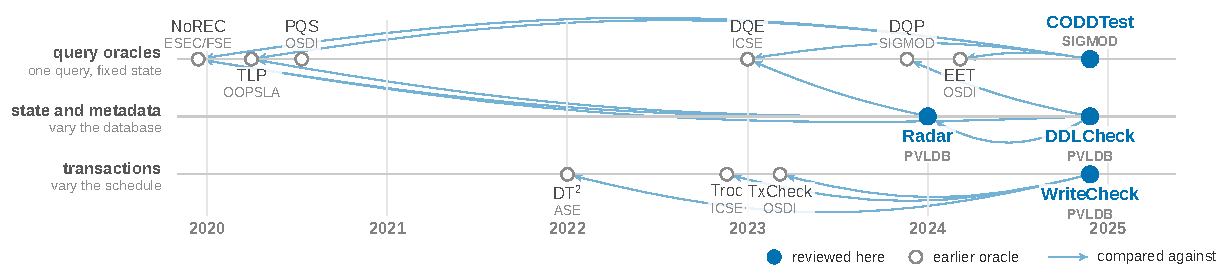
\includegraphics[width=\linewidth]{fig_lineage}
\caption{\textbf{Where the four papers sit in the oracle family, 2020--2025.} Lanes group oracles by what they vary; arcs point from each reviewed paper to the earlier tools it compares against in its evaluation. Venues from the papers' reference lists.}
\label{fig:lineage}
\end{figure*}

\begin{takeaway}
The four oracles are complements. Each sees a failure class the others cannot, and none sees a bug that corrupts both of its runs.
\end{takeaway}

% sec_b.tex: Experimental study, Discussion, Conclusions

\section{Experimental study}\label{sec:experiments}
All four papers make a solid case that their oracles work in practice, yet the strength of their experimental backing varies sharply across claims. Below we summarize the shared setup, review each paper's experimental procedures and results, and grade its claims using the symbols from Table~\ref{tab:coverage}: \yes\ for solid support, \half\ for directional or conditional evidence, and \no\ when the published evidence does not establish the claim.

\subsection{Setup, datasets and metrics}
\paragraph{Setup.} Table~\ref{tab:glance} summarizes the four setups. All four tools are written in Java: CODDTest, Radar and WriteCheck extend SQLancer, while DDLCheck is standalone. Where deployment is described, client-server engines run in Docker or from official binaries, with SQLite embedded. DDLCheck, Radar and WriteCheck used 8-core, 32\,GB hosts; CODDTest's efficiency study used a 64-core, 512\,GB server with 10 threads per configuration. Because engine versions, budgets and baselines vary across papers (and authors upgraded builds mid-campaign), raw counts across studies reflect setup as much as oracle quality. We therefore compare quantitative numbers strictly within each paper.

\begin{table*}[!tb]
\caption{\textbf{Experimental setup of the four studies,} taken from each paper's evaluation section. Engine versions identify evaluation snapshots; development campaigns could upgrade builds. Generator defaults list upper limits per generated test case.}
\label{tab:glance}
\centering\footnotesize\renewcommand{\arraystretch}{1.12}
\begin{tabularx}{\linewidth}{@{}l>{\raggedright\arraybackslash}X>{\raggedright\arraybackslash}p{3.5cm}>{\raggedright\arraybackslash}p{3.1cm}>{\raggedright\arraybackslash}p{3.5cm}@{}}
\toprule
\textbf{Study} & \textbf{DBMSs and versions} & \textbf{Deployment and hardware} & \textbf{Discovery budget} & \textbf{Generator defaults} \\
\midrule
CODDTest & SQLite, MySQL, CockroachDB, DuckDB, TiDB (development versions); SQLite 3.42.0.0 and 3.30.0 for comparisons & 64 cores, 512\,GB, 10 threads (efficiency study) & Intermittent runs over four months; 24\,h per comparison & Expression depth 3 (sweep 1 to 15) \\
DDLCheck & MySQL 8.0.36, PostgreSQL 16.2, SQLite 3.43.0, MariaDB 11.3.2, CockroachDB 23.2, TiDB 8.0.0 & 8 cores, 32\,GB; Docker or official binaries & 24\,h per DBMS & Max DDL length 10; 5,000 statements per DB pair \\
Radar & MySQL 8.0.32, SQLite 3.41.0, MariaDB 11.0.3, CockroachDB 22.2.5, TiDB 6.6.0 & 8 cores, 32\,GB; three-node CockroachDB, distributed TiDB & 10 rounds of 24\,h per DBMS & 3 tables, 3 columns, 30 rows, 5 indexes, 3 foreign keys \\
WriteCheck & MySQL 8.0.32, PostgreSQL 15.2, SQLite 3.36.0, MariaDB 10.11.2, CockroachDB 22.2.5, TiDB 6.6.0 & 8 cores, 32\,GB; single-node CockroachDB & 5 rounds of about 24\,h & Up to 5 transactions, 5 statements each; 2\,s client wait \\
\bottomrule
\end{tabularx}
\end{table*}

\paragraph{Datasets.} None of the papers uses a common standard benchmark; their generated test inputs are synthetic: SQLancer tables and expressions in CODDTest, random DDL chains and DML in DDLCheck, typed tables with constraints and indexes in Radar, and small typed tables with up to five explicit and autocommit transactions in WriteCheck. Synthetic generation fits semantic testing well. Correctness depends on SQL rules rather than domain data, fuzzing reaches unusual type, NULL and constraint combinations, and tiny databases keep counterexamples short enough to reduce. The cost is that none of the experiments says how these tools behave on large production databases.

WriteCheck additionally uses a systematic study of historical transaction bugs to motivate its design and calibrate generator bounds. Its authors studied 140 transaction bugs filed from 2018 to 2022, identifying 35 critical bugs that leave wrong data behind, of which 32 (91.4\%) violate WSS~\cite{writecheck}. Those 32 real defects are strikingly small~\cite[Fig.~2]{writecheck}: all need at most two tables and five transactions, 97\% of their initial tables have at most five rows, and 72\% require a specific key, index or column constraint. Historical bugs thus validate the oracle and calibrate generator bounds, while synthetic fuzzing finds new defects. Confirmed bug sets in the capability studies below provide a second source of real data.

\paragraph{Metrics and methodology.} Unique confirmed bugs serve as the headline metric, since developer confirmation is the clearest proof a finding is real, though counts still depend on how strictly authors reduce and deduplicate reports. Cost is measured as tests or queries per unit time. Two diversity proxies also appear: unique query plans in CODDTest (motivated by prior work linking plan diversity to bugs) and unique schema structures in DDLCheck. Code coverage is reported too, yet reveals little here: SQLite's own test suite reaches 100\% branch coverage while still shipping logic bugs~\cite[Sec.~4.3]{coddtest}.

Baseline comparisons take two distinct forms. A \textbf{capability study} fixes a set of known bugs and asks whether each tool could expose them. A \textbf{fresh run} gives every tool the same wall-clock budget to generate its own tests and counts what each finds. None of the papers reports variance or confidence intervals: comparative runs and ablations are single trials, and Radar's ten and WriteCheck's five discovery rounds report only totals.

\subsection{CODDTest results}
\paragraph{Procedure.} CODDTest obtains an expression's value through an auxiliary query and substitutes that value into the original query while preserving SQL context. Its efficiency benchmark separates expression-only, subquery-only and full modes, using separate matched 24-hour runs to measure throughput and to collect distinct query plans and branch coverage. The depth sweep varies \texttt{MaxDepth} from 1 to 15 in expression-only mode under a fixed 24-hour budget to isolate expression complexity~\cite[Sec.~4.3]{coddtest}.

CODDTest reports four series: an intermittent four-month campaign on five DBMSs; an oracle comparison combining a fresh run on SQLite 3.30.0, bug-age tracking and a manual detectability check; an efficiency benchmark against NoREC, TLP, DQE and two CODDTest variants; and the expression-depth sweep. Default runs use depth 3, 24 hours and 10 threads.

Across five DBMSs, CODDTest found 45 new bugs, including 24 logic bugs (19 fixed and 5 verified at publication). In the authors' manual breakdown, 11 of those 24 involve constructs earlier oracles omit, such as subqueries, \texttt{ON} clauses and \texttt{CASE} expressions~\cite[Table~2]{coddtest}.

\begin{figure}[!tb]
\centering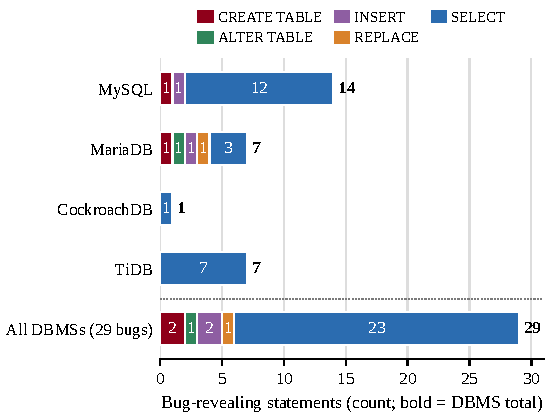
\includegraphics[width=\columnwidth]{fig4}
\caption{\textbf{Tests versus unique query plans in 24 hours} on SQLite 3.42.0.0, one point per mode, from \cite[Table~3]{coddtest}. Throughput and plans come from separate matched runs; branch coverage is 62--64\% except DQE (46.7\%).}
\label{fig:efficiency}
\end{figure}

Figure~\ref{fig:efficiency} shows the throughput-versus-diversity trade-off. Because each case runs at least three queries, CODDTest completes 4.20 times fewer tests than NoREC and 1.96 times fewer than TLP in 24 hours, yet reaches roughly 15 times more unique query plans. Branch coverage sits at 62--64\% for every variant except DQE and misses this 15-fold gap completely. CODDTest's standalone variants show the source: expression-only runs fastest among CODDTest modes (1.42 billion tests) yet hits just 7,399 plans, whereas subquery-only hits 2.76 million plans versus 2.58 million for the full mode. In Figure~\ref{fig:depth}, raising maximum depth from 1 to 15 pushes per-query time up 9.91 times, cuts throughput by 89.4\% and shrinks unique plans. The sweep measures runtime cost clearly, yet never tests whether deeper expressions find bugs shallow ones miss.

\begin{figure}[!tb]
\centering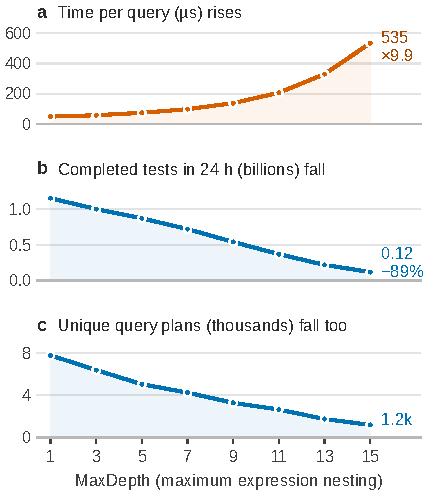
\includegraphics[width=\columnwidth]{fig_depth}
\caption{\textbf{Cost of CODDTest's expression-only mode as maximum expression depth increases,} one 24-hour run per depth, normalized to depth 1. Curves read from \cite[Figs.~2 and~3]{coddtest} (approximate); endpoint labels use the paper's reported values.}
\label{fig:depth}
\end{figure}

In the fresh 24-hour run on SQLite 3.30.0 (an older build where NoREC and TLP had already found 31 bugs), CODDTest found 25 unique bugs, trailing the 27 found by both NoREC and TLP, though it caught more exclusive bugs than any rival (4 versus 3 for NoREC and EET and 2 for TLP; Table~\ref{tab:fresh}).

\begin{verdicts}
\verdict{\yes}{CODDTest uncovers new logic bugs in mature engines.}{24 confirmed logic bugs across five DBMSs, 19 fixed.}
\verdict{\half}{It reaches bugs earlier oracles miss.}{The 11-of-24 count is measured on its own bugs (Figure~\ref{fig:homeset}); the fresh run shows complementarity, not superiority.}
\verdict{\no}{Deeper expressions are unnecessary.}{The depth sweep establishes runtime cost, not bug yield by depth.}
\end{verdicts}

\subsection{DDLCheck results}
\paragraph{Procedure.} DDLCheck executes a generated DDL sequence (up to length 10), extracts the resulting schema from the catalog and synthesizes a direct \texttt{CREATE} twin. It then runs the same generated DML and DQL statements on both databases, comparing query output, statement status, stored data and schema state. Its optimization records a database schema transition graph whose nodes hold table structures and whose edges represent DDL transitions; a new sequence is skipped if an equivalent graph (matching structural attributes and transition types up to column renaming) was already tested. This acts as a novelty filter rather than a numerical ranker, and the ablation varies this filter under a fixed 24-hour budget~\cite[Secs.~3.5, 4.4]{ddlcheck}.

DDLCheck presents a 24-hour-per-DBMS campaign across six engines, an ablation of its schema-diversity filter, and a conceptual check of whether NoREC, Radar and DQP could catch its confirmed schema bugs. Its default of 5,000 statements per database pair came from a pilot that also tested 25,000 and 100,000.

The campaign submitted 34 reports and earned 29 confirmations (21 schema logic bugs and 8 crashes), with zero false positives, 4 duplicates and 9 fixes~\cite[Table~2]{ddlcheck}. Seven of the 21 logic bugs never altered a query result: four corrupted stored data and three corrupted the schema. Across all 29 confirmed bugs, \texttt{SELECT} revealed 23 while \texttt{CREATE} (2), \texttt{INSERT} (2), \texttt{ALTER} (1) and \texttt{REPLACE} (1) exposed six~\cite[Fig.~6]{ddlcheck}, showing why checking only \texttt{SELECT} results is insufficient. In the conceptual comparison, NoREC exposed 0 of the 21 schema bugs, Radar 13 and DQP 9. In the ablation, keeping only DDL sequences yielding unseen schema structures raised unique bugs from 5 (random selection) to 8 (Figure~\ref{fig:ablation}b); a stricter filter triggered the same 9 raw failures but only 4 unique bugs.

\begin{verdicts}
\verdict{\yes}{Schema history exposes defects query oracles miss.}{29 confirmed bugs, zero false positives and 7 invisible to query output.}
\verdict{\half}{The diversity filter improves discovery.}{8 unique bugs against 5, from one 24-hour run per DBMS.}
\verdict{\no}{Effective testing of PostgreSQL and SQLite.}{Zero bugs in 24 hours cannot separate bug-free engines from generator limits.}
\end{verdicts}

\subsection{Radar results}
\paragraph{Procedure.} Radar abstracts database metadata by stripping table and column names and replacing column references inside constraints with their data types. A generated database is tested only when its abstract metadata pattern is unseen, after which the pattern is recorded. Radar then builds a raw twin retaining compulsory metadata and stored rows, runs up to 5,000 read queries on both databases and compares returned rows (ignoring order) and errors. The ablation disables the novelty filter while holding the rest of the pipeline fixed~\cite[Secs.~3.1, 3.4--3.5, 4.3]{radar}.

Radar reports ten 24-hour discovery rounds per DBMS on five systems, a 12-hour ablation of metadata-guided generation with function coverage, and a comparison against DQE, NoREC, TLP and MutaSQL combining conceptual analysis with a fresh 12-hour run (omitting MutaSQL, which is not public).

Ten rounds produced 1,663 raw reports. Roughly three weeks of manual reduction distilled them into 42 unique submissions: 38 confirmed (30 metadata-related, 8 other), 1 duplicate and 3 false positives~\cite[Sec.~4.2]{radar}. TiDB accounts for 31 of the 42 submissions and 24 of the 30 metadata bugs~\cite[Table~2]{radar}. Radar's guidance ablation (Figure~\ref{fig:ablation}a) provides a direct within-tool comparison: on TiDB, guided fuzzing separates within two hours and ends at 19 unique bugs versus 12. Across all five DBMSs the totals are 22 versus 14, so TiDB supplies most of the gain. Function coverage barely moves (20.3\% versus 19.7\% on MySQL; 19.7\% versus 19.3\% on MariaDB). In the fresh 12-hour run, all tools combined found 21 metadata bugs; Radar found 20, including 15 missed by every baseline.

\begin{figure}[!tb]
\centering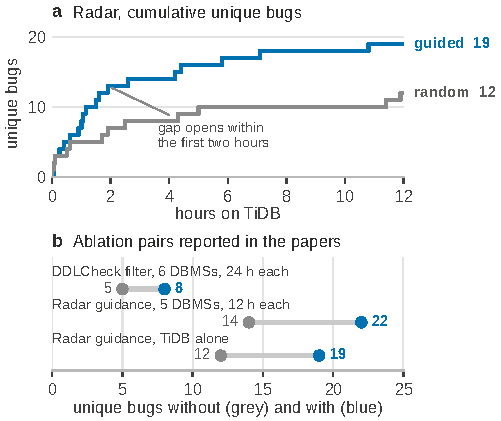
\includegraphics[width=\columnwidth]{fig_ablation}
\caption{\textbf{Ablation results from DDLCheck and Radar.} (a) Radar on TiDB: cumulative unique bugs with and without metadata guidance, read from \cite[Fig.~7]{radar} (approximate). (b) Total unique bugs with and without each design choice, from \cite[Table~3]{ddlcheck} and \cite[Table~3]{radar}. Each bar comes from a single run; differing targets and budgets preclude cross-tool ranking.}
\label{fig:ablation}
\end{figure}

\begin{verdicts}
\verdict{\yes}{Raw copies uncover metadata bugs other oracles miss.}{15 of 21 metadata bugs in the fresh run were found by Radar alone.}
\verdict{\half}{Metadata guidance improves detection.}{22 versus 14 bugs in a single run, concentrated in TiDB.}
\verdict{\half}{Findings generalize evenly across DBMSs.}{24 of the 30 confirmed metadata bugs come from one system.}
\end{verdicts}

\subsection{WriteCheck results}
\paragraph{Procedure.} WriteCheck randomly interleaves statements across concurrent transactions while preserving intra-transaction order. Each submitted statement runs in its own thread, and the client waits up to 2\,s before classifying a transaction as blocked so other eligible transactions can proceed; this client threshold is not an engine lock-wait timeout and does not by itself prove deadlock. Error recovery follows engine semantics: deadlock victims abort automatically in MySQL and TiDB, whereas SQLite, MariaDB, PostgreSQL and CockroachDB require an explicit \texttt{ROLLBACK} after relevant transaction errors. Serial replay is inferred from observed commit, rollback and abort events rather than submission order~\cite[Secs.~5.2--5.4]{writecheck}.

WriteCheck backs its oracle with the historical study of 35 critical bugs, a five-round campaign on six DBMSs, a capability comparison on 29 known bugs, and a fresh 12-hour run against DT\textsuperscript{2}, Troc and TxCheck.

The historical study anchors the design: 32 of 35 critical bugs (91.4\%) violate WSS, and 29 of those 32 (90.6\%) trigger deterministically under controlled statement order. Breaking down the two variants, 15 of the 35 critical bugs violate \texttt{tx-WSS} whereas 32 violate \texttt{stmt-WSS} (including all 15 \texttt{tx-WSS} cases)~\cite[Sec.~3.2]{writecheck}, demonstrating why checking whole-transaction replay alone misses defects exposed by statement-level replay.

Discovery flagged 101 WSS violations that reduced to 22 unique cases: 13 confirmed critical bugs (11 new, 2 known: 9 in TiDB, 3 in MariaDB, 1 in MySQL) and 9 false positives. One detail requires care: the capability study also evaluates 29 bugs, yet it is a \emph{different} set of 29, combining WriteCheck's 13 bugs with 16 found earlier by DT\textsuperscript{2}, Troc and TxCheck~\cite[Sec.~6.5.1]{writecheck}. WriteCheck detects all 29, versus 23 for DT\textsuperscript{2}, 16 for TxCheck, 14 for Troc and 0 for Elle, Cobra and Emme (Figure~\ref{fig:homeset}). Because most cases come from competing tools, this study is less restricted to the new tool's own discoveries than the other three capability studies. In the fresh 12-hour run (Table~\ref{tab:fresh}), WriteCheck found 4 critical bugs against 1 or 2 for each baseline, while rivals also catch non-critical bugs outside WriteCheck's main WSS target. WriteCheck's separate Serializable read-result check (excluding PostgreSQL) found no bugs in the evaluation.

\begin{table}[!tb]
\caption{\textbf{Results of the fresh end-to-end comparisons.} Unique bugs discovered, with exclusive finds in parentheses and false positives after the slash. Counts must not be interpreted as a ranking across papers. From \cite[Sec.~4.2]{coddtest}, \cite[Table~6]{radar} and \cite[Table~4]{writecheck}.}
\label{tab:fresh}
\centering\footnotesize\setlength{\tabcolsep}{3pt}
\begin{tabularx}{\columnwidth}{@{}>{\raggedright\arraybackslash}p{1.95cm}>{\raggedright\arraybackslash}p{1.55cm}>{\raggedright\arraybackslash}X@{}}
\toprule
\textbf{Run} & \textbf{Reviewed tool} & \textbf{Baselines} \\
\midrule
CODDTest, SQLite, 24\,h & 25 (4); 14/39 missed & NoREC 27 (3), TLP 27 (2), EET 6 (3) \\
Radar, 12\,h per DBMS & 20 of 21 (15) & all others together: 6 \\
WriteCheck, 12\,h per DBMS & 4 / 5 FP & DT\textsuperscript{2} 2 / 24, Troc 2 / 4, TxCheck 1 / 4 \\
\bottomrule
\end{tabularx}
\end{table}

\begin{verdicts}
\verdict{\yes}{WSS captures most critical transaction bugs.}{32 of 35 historical defects, drawn independently, violate it.}
\verdict{\half}{WriteCheck beats earlier transaction testers.}{29 versus at most 23 on the mixed capability set, and 4 versus 2 in one run; counts are small.}
\verdict{\half}{A WSS violation reliably signals a bug.}{9 of 22 unique discovery violations (and 5 in the 12-hour run) were false positives from semi-consistent reads and missing gap locks.}
\end{verdicts}

\paragraph{What the experiments prove.} A clear divide runs through all four studies. Discovery campaigns show that each oracle finds real bugs maintainers confirm and fix, and capability studies show many of those bugs lie outside older oracles' reach. Claims about \emph{how much} better one tool is than another rest on thinner ground: fresh runs and ablations use single trials with small counts, CODDTest trails NoREC and TLP in raw SQLite totals, and code coverage fails to separate configurations whose plan diversity differs 15-fold.

\section{Cross-study discussion and threats to validity}\label{sec:discussion}
Each paper reads well on its own. Side by side, three reporting habits blur any direct ranking by bug count, and none stands out until all four papers are read together.

\begin{figure*}[!tb]
\centering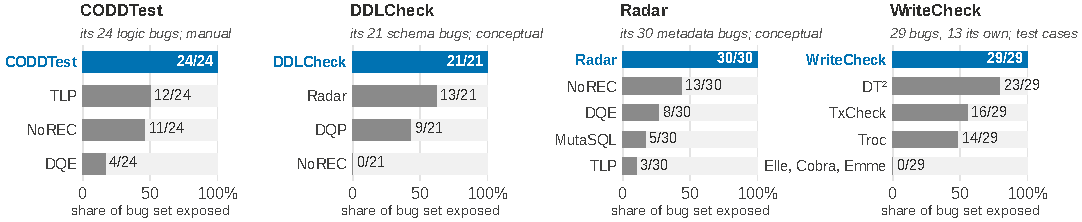
\includegraphics[width=\linewidth]{fig_homeset}
\caption{\textbf{Capability studies across the four papers.} Each panel measures what share of one paper's bug set every tool can detect, as judged by that paper's authors. In the first three panels, the bug set contains only the reviewed tool's own discoveries, so that tool scores 100\% by construction. WriteCheck's set combines its 13 bugs with 16 found by competing tools. From \cite[Table~2]{coddtest}, \cite[Table~4]{ddlcheck}, \cite[Table~5]{radar} and \cite[Table~3]{writecheck}.}
\label{fig:homeset}
\end{figure*}

\paragraph{Capability studies on the tool's own bugs.} Three of the four capability studies take the new tool's discoveries and ask how many older tools could catch them (Figure~\ref{fig:homeset}), guaranteeing the new tool 100\% by construction. That proves the new oracle reaches fresh territory, yet leaves the mirror question untouched: what does the new tool miss? Fresh comparisons partly answer that side: CODDTest missed 14 of 39 bugs found collectively in its SQLite experiment, while Radar missed 1 of 21 metadata bugs in its separate comparison. Because these fractions span different bug classes, targets and budgets, they cannot establish an overall ranking.

\paragraph{Headline counts from different triage stages.} Figure~\ref{fig:units} draws each reported item as one square colored by triage outcome. Every abstract highlights its row total, yet those totals represent different stages: all 45 of CODDTest's bugs are confirmed, DDLCheck's 34 reports include 4 duplicates and 1 awaiting confirmation, Radar's 42 submissions include 1 duplicate and 3 false positives, and WriteCheck's 22 unique violations include 2 known bugs and 9 false positives. Ranking abstract totals mixes confirmed fixes with duplicates and false alarms. Confirmation counts are also frozen at submission, and overlap across the four campaigns is unchecked.

\begin{figure}[!tb]
\centering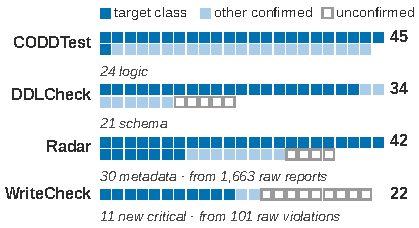
\includegraphics[width=\columnwidth]{fig_units}
\caption{\textbf{Breakdown of each paper's headline count by triage status.} Each square represents one reported case; row totals match each abstract. WriteCheck's 2 known bugs are confirmed duplicates; DDLCheck has 1 report awaiting confirmation. From \cite[Table~1]{coddtest}, \cite[Table~2]{ddlcheck}, \cite[Table~2]{radar} and \cite[Table~2]{writecheck}.}
\label{fig:units}
\end{figure}

\paragraph{The uncounted labor of triage.} Every unique bug starts inside a pile of raw failures someone must reduce and deduplicate. Figure~\ref{fig:triage} aligns the reported ratios: in CODDTest's SQLite run, NoREC and TLP emitted over 3,500 raw reports per unique bug, CODDTest about 280 and EET under 3; Radar averaged around 40 reports per bug and three weeks of manual work, while WriteCheck averaged about 5. Those ratios span three orders of magnitude, yet only Radar reports how long triage took. Flooding engineers with thousands of duplicates per real bug carries a steep operational cost that headline counts hide.

\begin{figure}[!tb]
\centering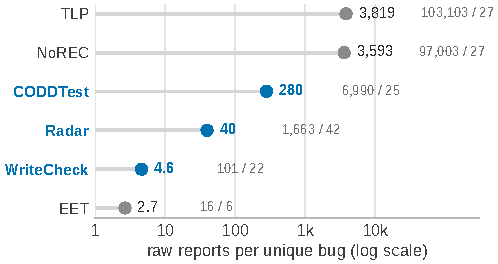
\includegraphics[width=\columnwidth]{fig_triage}
\caption{\textbf{Raw reports per unique bug,} with raw totals shown on the right. From \cite[Sec.~4.2]{coddtest}, \cite[Sec.~4.2]{radar} and \cite[Sec.~6.2]{writecheck}. Run durations, targets and triage definitions differ; ratios illustrate reported workload rather than a ranking of triage efficiency.}
\label{fig:triage}
\end{figure}

\paragraph{Evidence summary.} Table~\ref{tab:scorecard} collects all verdicts: the top two rows hold across all four papers, while the comparative claims below remain directional or conditional at best.


\paragraph{Threats to validity.} Internal validity rests on precondition soundness: stray nondeterminism, implicit casts or incomplete catalog reconstruction trigger mismatches without any DBMS bug. Construct validity is limited because distinct query plans do not ensure distinct semantic paths, and 100\% branch coverage still coexists with logic bugs in SQLite~\cite[Sec.~4.3]{coddtest}. External validity faces four constraints: deployments differ even for one engine (single-node CockroachDB in WriteCheck versus a three-node cluster in Radar), small generated tables differ from long-lived production databases, three of the four papers (DDLCheck, Radar and WriteCheck) originate from the same research group and three (CODDTest, Radar and WriteCheck) share the SQLancer framework, and bug finds cluster unevenly. In Figure~\ref{fig:dbms}, CODDTest's logic bugs are distributed more broadly across its targets; DDLCheck clusters in MySQL and MariaDB, while Radar and WriteCheck concentrate in TiDB. Because none of the papers separates dialect fit, engineering effort and maturity, Figure~\ref{fig:dbms} does not rank DBMS reliability.

\begin{figure}[!tb]
\centering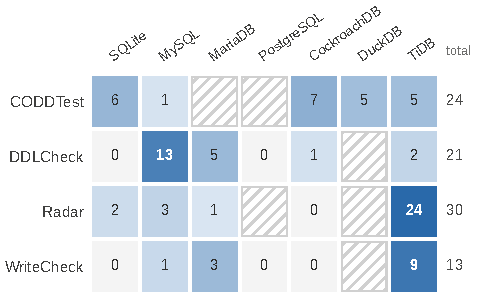
\includegraphics[width=\columnwidth]{fig_dbms}
\caption{\textbf{Target bugs per campaign by DBMS.} Shading shows each engine's share; hatched cells were not tested. Counts are logic bugs (CODDTest), schema bugs (DDLCheck), metadata bugs (Radar) and critical bugs (WriteCheck), from \cite[Table~1]{coddtest}, \cite[Table~2]{ddlcheck}, \cite[Table~2]{radar} and \cite[Table~3]{writecheck}.}
\label{fig:dbms}
\end{figure}


\section{Conclusions and research directions}\label{sec:conclusions}

\begin{table*}[!tb]
\caption{\textbf{Strength of evidence for recurring claims across the four papers.} Our assessment of the published record.}
\label{tab:scorecard}
\centering\small\renewcommand{\arraystretch}{1.12}
\begin{tabularx}{\linewidth}{@{}>{\raggedright\arraybackslash}p{4.9cm}*{4}{>{\centering\arraybackslash}p{1.15cm}}>{\raggedright\arraybackslash}X@{}}
\toprule
\textbf{Claim} & \textbf{\shortstack{CODD-\\Test}} & \textbf{\shortstack{DDL-\\Check}} & \textbf{\shortstack{\strut\\Radar}} & \textbf{\shortstack{Write-\\Check}} & \textbf{Main qualification} \\
\midrule
Finds new bugs that developers confirm & \yes & \yes & \yes & \yes & Publication snapshots; cross-campaign overlap unknown \\
Reaches bugs that earlier oracles miss & \yes & \yes & \yes & \yes & Three sets use own bugs (Fig.~\ref{fig:homeset}); WriteCheck uses a mixed set \\
Finds more bugs than baselines in a fresh run & \no & \nt & \half & \half & Single runs, small counts; different targets and bug classes \\
Generation or design choice helps & \half & \half & \half & \half & Single runs; CODDTest sweep tests cost, not bug yield \\
False alarms are characterized & \half & \yes & \yes & \yes & CODDTest notes causes without initial count; WriteCheck quantifies FPs \\
Effectiveness generalizes across DBMSs & \yes & \half & \half & \half & Radar 24/30 and WriteCheck 9/13 in TiDB; zeros may reflect generators \\
Repeated-run uncertainty is reported & \no & \no & \no & \no & 10 and 5 rounds run, no spread or confidence intervals given \\
\bottomrule
\end{tabularx}
\symkey{\yes/supported, \half/{directional, small or conditional}, \no/not established, \nt/not tested}
\end{table*}

Read together, these papers suggest a modular testing suite built from independent oracles: CODDTest for expressions, DDLCheck for schema history, Radar for metadata and WriteCheck for concurrent writes. Returning to our shop's \texttt{Product} table, such a suite would check folded stock predicates with CODDTest, validate \texttt{ALTER TABLE} migrations with DDLCheck, audit stock-index queries against a raw copy with Radar, and replay concurrent checkouts with WriteCheck. Keeping them separate ties every failure to one invariant; chaining them, such as running CODDTest or Radar over DDLCheck schemas, needs its own soundness proof.

\paragraph{Open questions.}
\begin{enumerate}[leftmargin=1.3em,itemsep=1pt,topsep=2pt]
\item \textbf{What should steer generation?} CODDTest's depth sweep shows that deeper syntax drives up cost without measuring bug yield, while DDLCheck's schema filter and Radar's metadata guidance point to unseen schema structures and metadata combinations.
\item \textbf{How can triage get cheaper?} Isolation names leave write semantics underspecified, and Radar still costs weeks of reduction; per-dialect profiles of valid transforms and locks could cut both.
\item \textbf{How can shared faults be caught?} Every oracle here uses the DBMS as its own referee; self-consistency checks narrow where bugs hide, yet identical faults on both paths still pass.
\end{enumerate}

\paragraph{Toward a neutral comparison.} Answering the open comparative questions requires a shared protocol: pin common DBMS revisions, build a neutral bug suite from independent historical reports (extending WriteCheck's start), and run all tools under equal budgets across multiple seeded trials. Report unique bugs with variance, false positives, raw reports per bug and triage time; include negative controls (valid tricky cases) to test precision; and score each oracle only on its claimed failure classes (Table~\ref{tab:coverage}).

\paragraph{Closing thoughts.} Each system opens a distinct layer of DBMS behavior to automated testing by pairing two executions expected to agree under explicit preconditions, and each rests on its precondition: stable evaluation for folding, a faithful catalog for reconstruction, metadata-agnostic queries for raw copies, and an obeyed conflict model for serial replay. Within those bounds, all four papers show convincingly that they catch bugs earlier oracles miss; comparing them under one neutral protocol is the clear next step.

\begin{thebibliography}{9}\footnotesize
\bibitem{coddtest} Chi Zhang and Manuel Rigger. 2025. Constant Optimization Driven Database System Testing. \emph{Proc.\ ACM on Management of Data} 3(1), Article 24, 1--24. \url{https://doi.org/10.1145/3709674}. Full text: \url{https://arxiv.org/pdf/2501.11252}.
\bibitem{ddlcheck} Jiansen Song, Wensheng Dou, Yingying Zheng, Yu Gao, Ziyu Cui, Wei Wang, and Jun Wei. 2025. Detecting Schema-Related Logic Bugs in Relational DBMSs via Equivalent Database Construction. \emph{Proc.\ VLDB Endowment} 18(7), 2281--2294. \url{https://doi.org/10.14778/3734839.3734861}. Full text: \url{https://www.vldb.org/pvldb/vol18/p2281-song.pdf}.
\bibitem{writecheck} Ziyu Cui, Wensheng Dou, Yu Gao, Rui Yang, Yingying Zheng, Jiansen Song, Yuan Feng, and Jun Wei. 2025. Simple Testing Can Expose Most Critical Transaction Bugs: Understanding and Detecting Write-Specific Serializability Violations in Database Systems. \emph{Proc.\ VLDB Endowment} 18(8), 2547--2560. \url{https://doi.org/10.14778/3742728.3742747}. Full text: \url{https://www.vldb.org/pvldb/vol18/p2547-cui.pdf}.
\bibitem{radar} Jiansen Song, Wensheng Dou, Yu Gao, Ziyu Cui, Yingying Zheng, Dong Wang, Wei Wang, Jun Wei, and Tao Huang. 2024. Detecting Metadata-Related Logic Bugs in Database Systems via Raw Database Construction. \emph{Proc.\ VLDB Endowment} 17(8), 1884--1897. \url{https://doi.org/10.14778/3659437.3659445}. Full text: \url{https://www.vldb.org/pvldb/vol17/p1884-song.pdf}.
\bibitem{norec} Manuel Rigger and Zhendong Su. 2020. Detecting Optimization Bugs in Database Engines via Non-Optimizing Reference Engine Construction. In \emph{Proc.\ ESEC/FSE 2020}, 1140--1152. \url{https://doi.org/10.1145/3368089.3409710}.
\bibitem{tlp} Manuel Rigger and Zhendong Su. 2020. Finding Bugs in Database Systems via Query Partitioning. \emph{Proc.\ ACM on Programming Languages} 4(OOPSLA), Article 211, 1--30. \url{https://doi.org/10.1145/3428279}.
\end{thebibliography}

\vspace{0.5em}
\paragraph{Disclosure of LLM use.}{\footnotesize Claude (Anthropic) drafted the \LaTeX{} conversion, figure scripts, explainer diagrams (TikZ), the reproduction runners and upstream patches, and prose edits. The authors chose the papers and arguments and ran the reproductions. They checked the cited numbers against the papers; values read off figures are approximate. An LLM-based review against the course guide was also used to find gaps.\par}

\end{document}
